
\begin{figure}
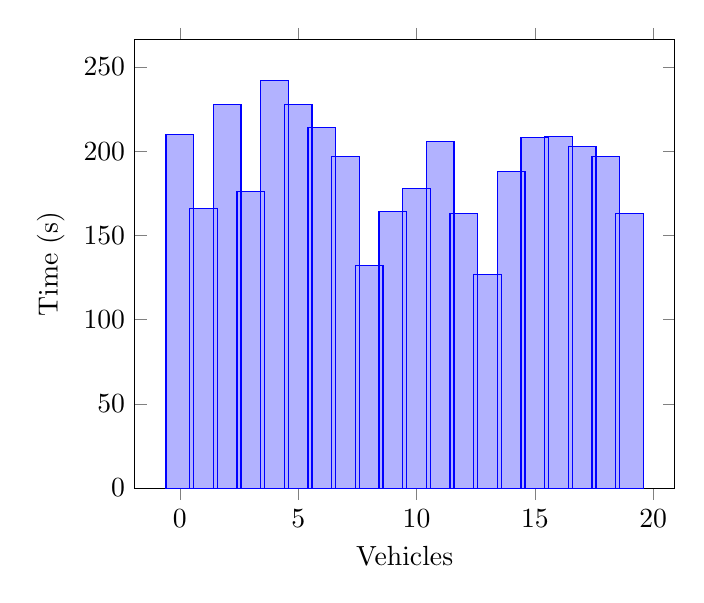
\begin{tikzpicture}
\begin{axis}[
legend style={anchor=west},
xlabel=Vehicles,
ylabel=Time (s),
ymin=0,
ybar,
]
\addplot coordinates {
(0, 210)
(1, 166)
(2, 228)
(3, 176)
(4, 242)
(5, 228)
(6, 214)
(7, 197)
(8, 132)
(9, 164)
(10, 178)
(11, 206)
(12, 163)
(13, 127)
(14, 188)
(15, 208)
(16, 209)
(17, 203)
(18, 197)
(19, 163)
};

\end{axis}
\end{tikzpicture}
\label{tik:0:2_O, 2_O.-60, 4_S, 5_S, 5_S.-30, 7_S, 7_S.-25, 11_S, 11_S.-50, 13_S, 15_N, 17_S, 17_S.-60, 20_O, 21_O}
\caption{0 percent diving with GSC on route $2_O, 2_O.-60, 4_S, 5_S, 5_S.-30, 7_S, 7_S.-25, 11_S, 11_S.-50, 13_S, 15_N, 17_S, 17_S.-60, 20_O, 21_O$}
\end{figure}
